\documentclass[fontsize=12pt,a4paper]{scrartcl}[2003/01/01]

\usepackage{listings}
\usepackage{courier}
\usepackage{graphicx}
\usepackage{float}

\title{Design of an UML tool with round-trip engineering for Java and implementation as a web application in Adobe Air}
\date{10.08.2011}
\author{Christoph Grundmann}

\begin{document}
\maketitle 
\tableofcontents 

\section{Round-trip engineering}
Today's complexity of software requires the use of diagrams that will describe the structure of programs and how the internal processes communicate, during and primary at the beginning of the development. Moreover for object oriented languages like Java, the UML standard is the way to go, because of its focus for the object oriented developing of software.  
Structure diagrams, like the class diagram, have the capability to generate source code by analyzing it. In addition it's possible to create a class diagram with the help of source code. 
The creation of Java source code from a class diagram is called forward engineering, whereas the creation of a class diagram from the Java source code is called reverse engineering. The whole technique is known as round trip engineering. So round trip engineering allows keeping the consistency between diagrams and source code.

\subsection{Reverse engineering}
To generate a class diagram with the help of Java source code, a parser is needed to interpret the grammatical structure of it. Usually a program doesn�t understand the grammatical structure of an input like a string before it is interpreted. The first step in interpreting the source code a parser converts it into a specific data format, in this case into a JSON object, which can use to interpret the grammatical structure. After that step the new output can be used to generate the class diagram. Classes can easily instantiate by reading the JavaScript friendly output, where the relations need to be interpreted.

\subsubsection{Parser}
AlphaUML uses �PEG.js�, a Java parser that is completely written in JavaScript, to parse Java source code into a JSON object. It allows converting a string, by using a specific language grammar, into any output format. The grammar describes the Java language and defines the output. It follows specific rules similar to regular expressions to match the input with the Java grammar. 
Furthermore it allows manipulating the output of each expression by using JavaScript as a so called �action�. In this case an action is used to convert the expression result to a JSON object. But in some cases an empty string returns if an expression is optional and it doesn�t match. Then the empty string will be replaced with null to catch missing matches in the processing to a class diagram.

\subsubsection{Parser grammar rules}
PEG.js provides some rules which are necessary to write an own grammar. A collection of the most common rules will be described below. In addition a small grammar example with explanation after the rules shows how they are used.

\paragraph*{\textbf{"literal" or 'literal'}}$\;$ \\
Return the literal string on matching.

\paragraph*{\textbf{.}}$\;$ \\
Return one character as a string.

\paragraph*{\textbf{\lbrack characters\rbrack}}$\;$ \\
Return one character of the bracket contained set.

\paragraph*{\textbf{rule}}$\;$ \\
It describes a fully expression that can use in other rules or expressions

\paragraph*{\textbf{(expression)}}$\;$ \\
It allows the declaration of a subexpression to encapsulate it. It�s similar to a rule and is necessary to set an expression optional.

\paragraph*{\textbf{expression *}}$\;$ \\
Zero or more match results allowed. Returns the result as an array.

\paragraph*{\textbf{expression +}}$\;$ \\
One or more match results necessary. If the input doesn't match it returns a parsing error.

\paragraph*{\textbf{expression ?}}$\;$ \\
It allows optional expressions. On succeeding the match result returns, otherwise it returns an empty string.

\paragraph*{\textbf{! expression}}$\;$ \\
It forbids a specific expression.

\paragraph*{\textbf{label : expression}}$\;$ \\
A label stores the match result into a specific variable that has the same name. It can be used in an action to get access of the stored result.

\paragraph*{\textbf{expression \{ action \}}}$\;$ \\
An action is a JavaScript snippet that will be executed 'cause the match is successful. It has the access to each labeled expression of its expression and allows the manipulation of the match result.

\paragraph*{\textbf{expression\_1 expression\_2 \dots expression\_n}}$\;$ \\
A sequence of expression is allowed and returns their results as an array.

\paragraph*{\textbf{expression\_1 / expression\_2 / \dots / expression\_n}}$\;$ \\
It allows to create an OR function. It tries to match with one of the given expressions.

\subsubsection{Parser grammar example}
The following example shows a rule called DataType which is used for parsing a data type. It matches primitive data types, generic types or array types. Each information will return as a JSON object, formatted by the action. The DataTypeKeyword rule provides a collection of data types and allows each possible java identifier (Identifier) as data type, so user-defined objects are possible. The Generic and Array rules are optional and return an empty string on miss.

\lstset{
	language=HTML, 
	numbers=left,
	numberstyle=\tiny,
	stepnumber=1
}

\begin{lstlisting}[caption={list of data type keywords}, frame=single]
DataTypeKeyword = (
        "boolean"
	/   "byte"
	/   "char"
	/   "double"
	/   "enum"
	/   "float"
	/   "int"
	/   "long"
	/   "short"
	/   "void"
	/   Identifier
)
\end{lstlisting}

\begin{lstlisting}[caption={data type rule}, frame=single]
DataType =
    $d:DataTypeKeyword __
    $g:($g:Generic __ {return $g;})?
    $a:($a:Array __ {return $a;})?
    {
        return {
            generic: $g !== "" ? $g : null,
            array: $a !== "" ? $a : false,
            dataType: $d
        };
    }
\end{lstlisting}

\subsubsection{Parser output}
\label{json} 
The produced output from the source code will be used to generate the class diagram. The JSON format of the output makes the next process easier, so it represents a specific logical structure and allows the immediate access to all necessary information about the parsed Java program.
The output provides, for example, the info about used libraries, the class package, all class methods or variables to generate the class diagram. In addition the JavaDoc is available and will be pinned as note at the specific class in the diagram.
The following JSON sample gives an overview about the output format and shows each possible fields like the �package� or �classes� fields.

\begin{lstlisting}[caption={file output}, frame=single]
{
   "package": "packageName",
   "imports": ["path"],
   "classes": []
}
\end{lstlisting}

\begin{lstlisting}[caption={classes output}, frame=single]
"classes": [
     {
        "type": "interface",
        "javaDoc": null,
        "visibility": "public",
        "name": "className",
        "extend": "superClass",
        "implement": [
            "interfaceName"
        ],
        "body": {
            "variable": [],
            "method": []
        }
    }
]
\end{lstlisting}

\begin{lstlisting}[caption={variable output}, frame=single]
"variable": [
    {
        "type": "variable",
        "javaDoc": null,
        "name": "varName",
        "visibility": "public",
        "modifier": [
            "static",
            "final"
        ],
        "array": false,
        "generic": null,
        "dataType": "int",
        "value": "42"
    }
]
\end{lstlisting}

\begin{lstlisting}[caption={method output}, frame=single]
"method": [
    {
        "type": "method",
        "javaDoc": {},
        "name": "methodName",
        "visibility": "public",
        "modifier": [],
        "generic": null,
        "array": true,
        "dataType": "String",
        "parameter": [
            {
                "type": "parameter",
                "modifier": ["static"],
                "generic": "T",
                "array": false,
                "dataType": "Object",
                "name": "paramterName"
            }
        ],
        "body": "methodBody"
    }
]
\end{lstlisting}

\begin{lstlisting}[caption={JavaDoc output}, frame=single]
"javaDoc": {
     "since": [
        {
           "tag": "since",
           "description": "desc"
        }
     ],
     "throws": [
        {
           "tag": "throws",
           "classname": "className",
           "description": "desc"
        }
     ],
     "exception": [
        {
           "tag": "exception",
           "classname": "className",
           "description": "desc"
        }
     ],
     "param": [
        {
           "tag": "param",
           "name": "paramName",
           "description": "desc"
        }
     ],
     "return": [
        {
           "tag": "return",
           "description": "desc"
        }
     ],
     "see": [
        {
           "tag": "see",
           "description": "desc"
        }
     ]
}
\end{lstlisting}

\subsubsection{Class diagram generation}


\subsection{Forward engineering}
To generate the source code from an existing class diagram, it�s essential to analyze each available class and connector, like generalizations or associations. The analyzing process will be handled from the classes themselves. So a class contains all necessary information and can handle it without an additional effort. Operations, parameter, attributes and classes own a method called \textit{getJSON()} that creates an output which is identical to the parser output \ref{json} and will be used to generate the source code. Furthermore it gets the relations between classes, so an additional process isn�t necessary. On getting each declared attribute, associations of the two classes and each required interface will be collected and set as attribute. Moreover if an interface extends another interface it will set as superclass and declare with the extend keyword, in the other case if a class provides an interface the implements keyword will be used. The following sections explain each available relation and their implementation. 

\subsubsection{Generalization}
If a class inherits from another class the subclass has to signalize the relation with the keyword �extends� in its declaration. In addition each operation and attribute which is declared in the superclass doesn�t need to be implemented into the subclass twice. If the user declares an operation which has the same name and parameter list of another one in the superclass, the superclass operation will be overwritten. To execute the method of the superclass Java contains the �super� keyword which is a reference on its class.

\begin{figure}[H]
\centering
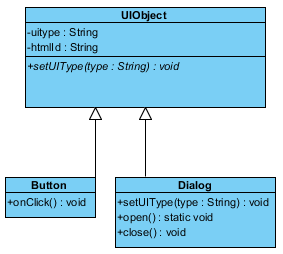
\includegraphics[scale=0.8]{images/example_generalization.png}
\caption{The class diagram shows the superclass �UIObject� and two subclasses which inherit from it. Moreover the class �Dialog� overrides the operation �setUIType� and implements some other methods.}
\end{figure}

\lstset{
	language=Java, 
	numbers=left,
	numberstyle=\tiny,
	stepnumber=1
}

\begin{lstlisting}[caption={The following code snippet shows the result of the code generation.}, frame=single]
public class UIObject {
	private String uitype;
	private String htmlId;
	
	public void setUIType(String type) {}
}

public class Button extends UIObject {
	public void onClick() {}
}

public class Dialog extends UIObject {
	public void setUIType(String type) {}

	public void open() {}

	public void close() {}
}
\end{lstlisting}

\subsubsection{Binary association}
A binary association specifies a semantic relationship between two classes. So two classes knew about the other one and can interact or communicate. An association provides a collection of properties, which are important to interpret for the code generation. 
First of all the multiplicity of a class defines the frequency of occurrence. If a multiplicity is declared as \lbrack 1..5\rbrack the class has to declare once and can be declared at most five time. In the source code a multiplicity represents an array if a class can declare more than one time, otherwise it�s a simple variable. Furthermore the role of a class gives the declaration of itself a specific name. So if a role is set the variable get the name of it. In addition it�s possible to set the visibility of a role. The last necessary association property is the navigation. An arrow visualizes the direction of the navigation and specify in which class the other one will be declared. The bidirectional navigation allows the navigation in both directions.

\subsubsection{Provided interfaces}
Provided interfaces are like generalizations with abstract classes. Each operation will be inherited and has to overwrite in the subclass. The only two differences are the �implements� keyword � instead of the �extends� keyword � which is use for inheritance and the fact that it�s possible to implement more than one interface. When using more than one interface, each interface will be separated by a comma, at its declaration.
An interface orders a specific realization of the class that inherits from it.

\subsubsection{Required interfaces}
A relation with required interfaces describes a dependency from these interfaces, which may not modify after implementation. So the class which implements a required interface gets access on the specific operations and attributes and would throw exceptions if one of those operations is changed. A required interface will be declared as an attribute and can be initialized by any constructor of classes which implement (provided interface) the interface.

\subsubsection{Extended interfaces}
If an interface will be extended, a generalization has to be used. That includes the UML generalization arrow and on the java side, the use of the �extends� keyword.

\end{document}